\documentclass[tikz,border=10pt]{standalone}
\begin{document}
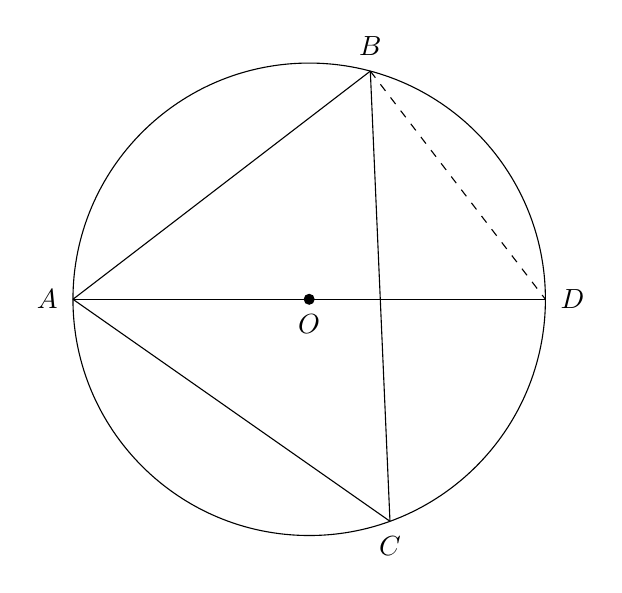
\begin{tikzpicture}[scale=2]
\coordinate (O) at (0,0);
\coordinate (A) at (-1.5,0);
\coordinate (D) at (1.5,0);
\coordinate (B) at (75:1.5);
\coordinate (C) at (290:1.5);

\draw (O) circle (1.5);
\draw (A) -- (D);
\draw (A) -- (B);
\draw (A) -- (C);
\draw (B) -- (C);
\draw[dashed] (B) -- (D);

\fill (O) circle (1pt);

\node[below=2pt] at (O) {$O$};
\node[left=2pt] at (A) {$A$};
\node[above=2pt] at (B) {$B$};
\node[below=2pt] at (C) {$C$};
\node[right=2pt] at (D) {$D$};
\end{tikzpicture}
\end{document}
